\documentclass{controle}
\usepackage{main}

\title{Évaluation n°16 : Variations de fonctions de références}
\author{Seconde 3}
\date{10 Avril 2026}

% \printanswers

\begin{document}
\titleandname{}
\version
\begin{questions}
\question[2] Compléter les phrases suivante :
\begin{parts}
\part La fonction carré est \dotfill sur $[0;+\infty[$.
\part La fonction racine carré est croissante sur \dotfill.
\end{parts}
\begin{solution}
\begin{parts}
\part La fonction carré est croissante sur $[0;+\infty[$.
\part La fonction racine carré est croissante sur $[0:+\infty[$.
\end{parts}
\end{solution}
\question[2] La fonction $x \mapsto -4x + 7$ est-elle croissante ou décroissante ?
\begin{solution}
Décroissante
\end{solution}
\question[6] Soit $f$ la fonction dont la courbe représentative est donné ci-dessous :
\begin{center}
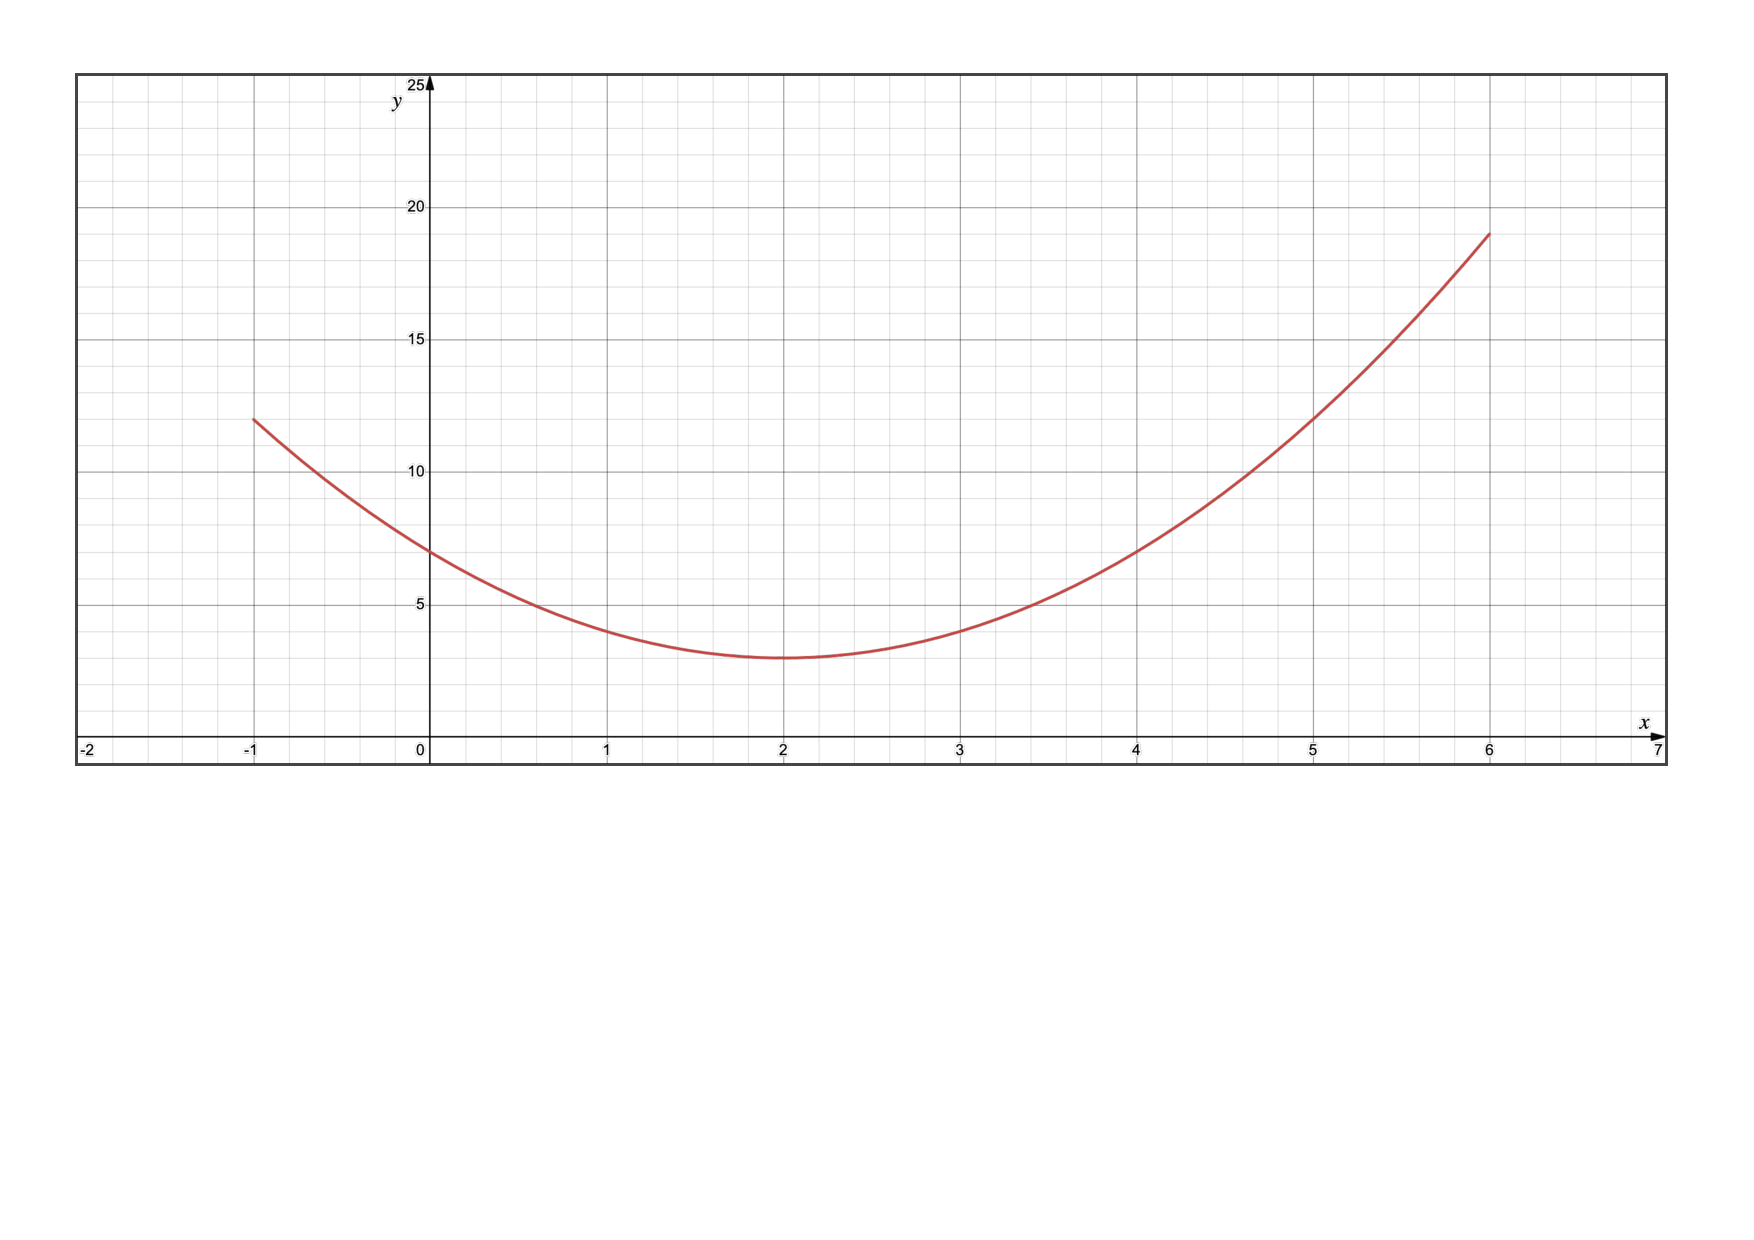
\includegraphics[width=0.8\textwidth,trim={0 8cm 0 1cm},clip]{Evaluation_16_Graph_v1.pdf}
\end{center}
Compléter le tableau de variation ci-dessous :
\begin{center}
\begin{tikzpicture}
\tkzTabInit{$x$ / 1, Variation de $f$ / 2}{$-1$,,$6$};
\end{tikzpicture}
\end{center}
\begin{solution}
\begin{center}
\begin{tikzpicture}
\tkzTabInit{$x$ / 1, Variation de $f$ / 2}{$-1$,$2$,$6$};
\tkzTabVar{+/$12$,-/$3$,+/$19$};
\end{tikzpicture}
\end{center}
\end{solution}
\end{questions}
\newpage
\titleandname{}
\version
\begin{questions}
\question[2] Compléter la phrase suivante :
\begin{parts}
\part La fonction carré est décroissante sur \dotfill.
\part La fonction cube est \dotfill sur $\R$.
\end{parts}
\begin{solution}
\begin{parts}
\part La fonction carré est décroissante sur $]-\infty;0]$.
\part La fonction cube est croissante sur $\R$.
\end{parts}
\end{solution}
\question[2] La fonction $x \mapsto 2x - 6$ est-elle croissante ou décroissante ?
\begin{solution}
Croissante
\end{solution}
\question[6] Soit $f$ la fonction dont la courbe représentative est donné ci-dessous :
\begin{center}
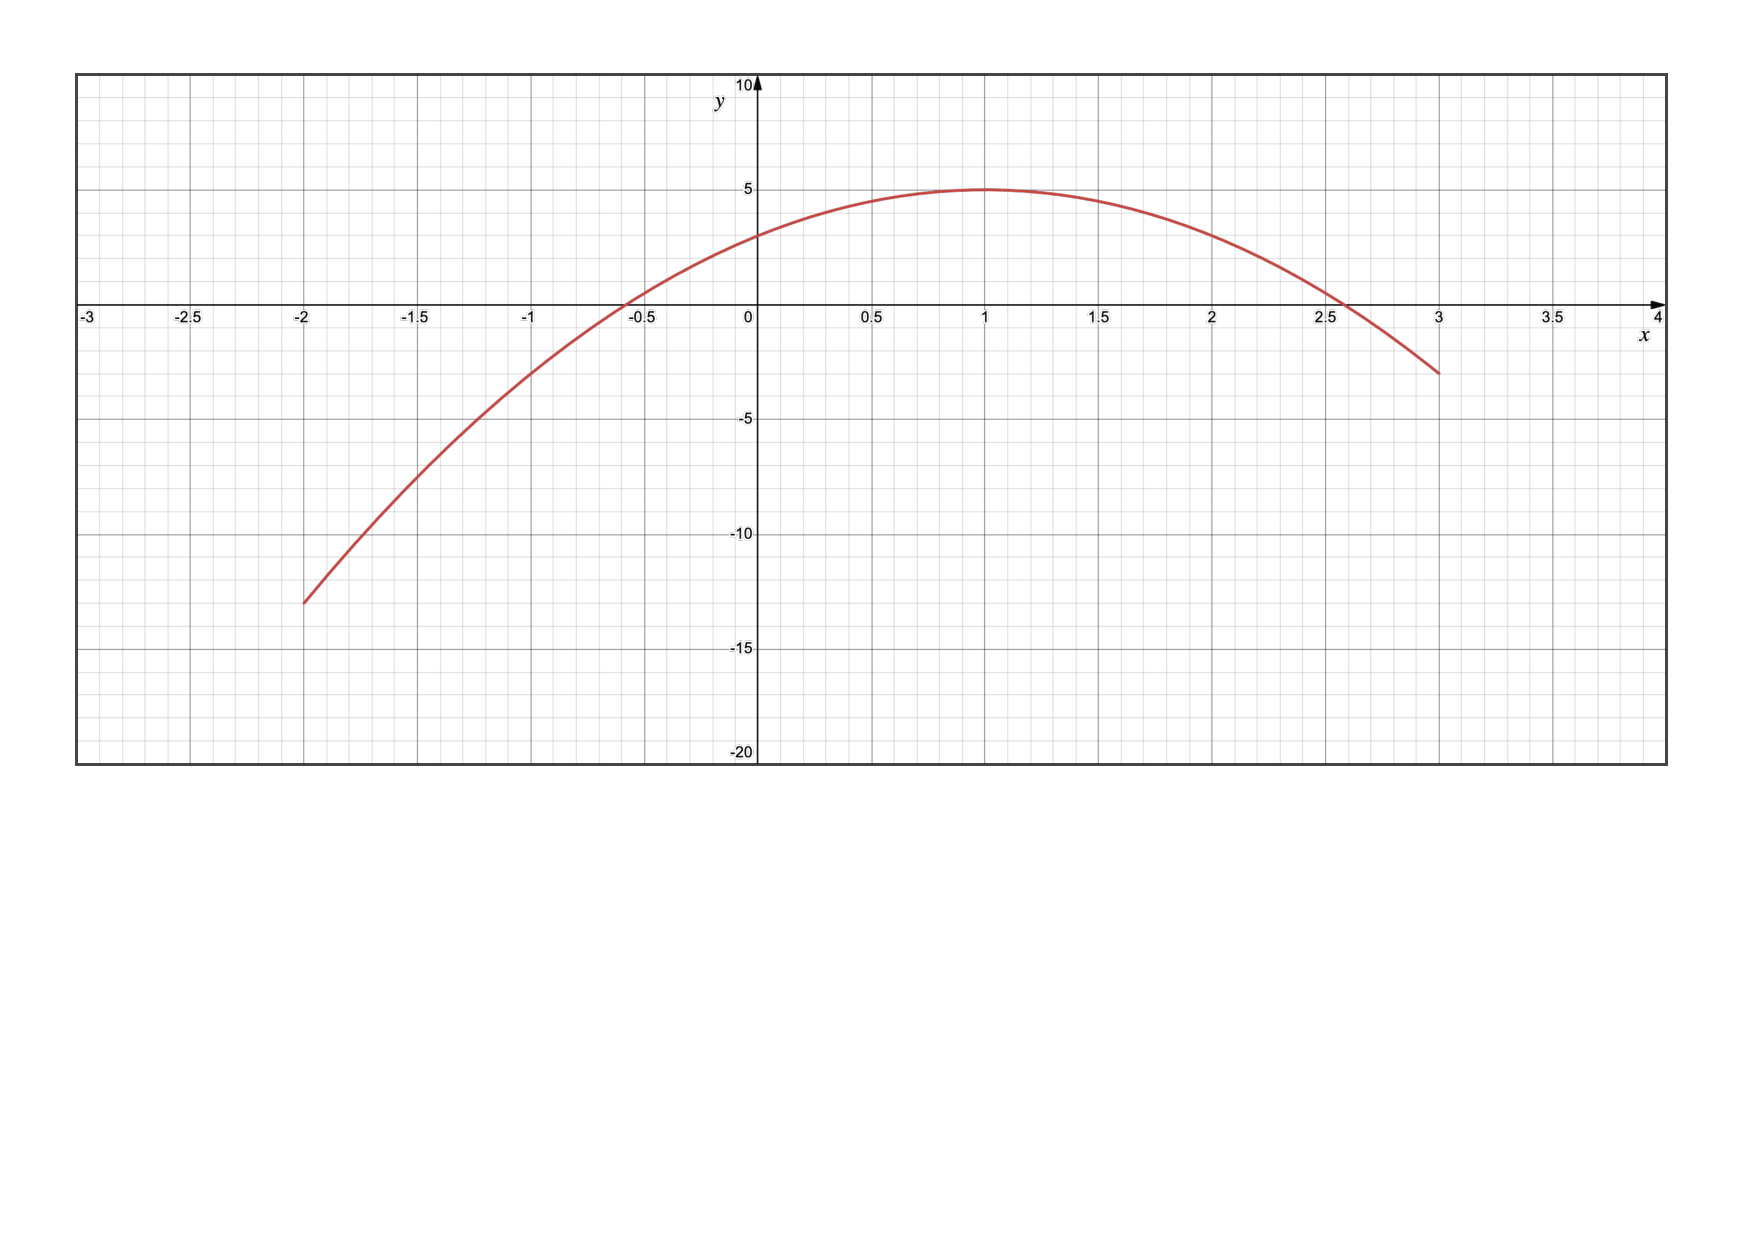
\includegraphics[width=0.8\textwidth,trim={0 8cm 0 1cm},clip]{Evaluation_16_Graph_v2.pdf}
\end{center}
Compléter le tableau de variation ci-dessous :
\begin{center}
\begin{tikzpicture}
\tkzTabInit{$x$ / 1, Variation de $f$ / 2}{$-2$,,$3$};
\end{tikzpicture}
\end{center}
\begin{solution}
\begin{center}
\begin{tikzpicture}
\tkzTabInit{$x$ / 1, Variation de $f$ / 2}{$-2$,$1$,$3$};
\tkzTabVar{-/$-13$,+/$5$,-/$-3$};
\end{tikzpicture}
\end{center}
\end{solution}
\end{questions}
\end{document}